\documentclass[8pt, landscape, fleqn]{scrartcl}
\setlength{\parindent}{0pt}
\usepackage[ngerman]{babel}
%\usepackage[applemac]{inputenc}
\usepackage[utf8]{inputenc}
\usepackage[dvips]{geometry}
\usepackage{latexsym}
\usepackage{multicol}
\usepackage{amsmath}
\usepackage{graphicx}
\usepackage{array}
\usepackage{booktabs}
\usepackage{amsmath}
\usepackage{mathtools}
\usepackage{ulem}
\usepackage{amsfonts}
\usepackage{dsfont}
\usepackage{charter} %%% Schreibart
%\renewcommand{\familydefault}{\sfdefault}



%%%%%%%%%%Paket für Chemische Formeln
\usepackage{chemformula} 
\usepackage[version=3]{mhchem}
%%%%%%%%%%%%%%%%% Farbe
\usepackage{color}

\pagestyle{plain}
\typearea{20}
\columnsep 30pt
\columnseprule .4pt
\setlength{\extrarowheight}{0.9em}

\renewcommand{\arraystretch}{0.8}

\makeatletter
\renewcommand{\section}{\@startsection{section}{1}{0mm}%
{-2\baselineskip}{0.8\baselineskip}%
{\hrule depth 0.2pt width\columnwidth\hrule depth1.5pt
width0.25\columnwidth\vspace*{1.2em}\Large\bfseries\rmfamily}}
\makeatother


\makeatletter
\renewcommand{\subsection}{\@startsection{subsection}{1}{0mm}%
{-2\baselineskip}{0.8\baselineskip}%
{\hrule depth 0.2pt width\columnwidth\hrule depth0.75pt
width0.25\columnwidth\vspace*{1.2em}\large\bfseries\rmfamily}}
\makeatother

\makeatletter
\renewcommand{\subsubsection}{\@startsection{subsubsection}{1}{0mm}%
{-2\baselineskip}{0.8\baselineskip}%
{\hrule depth 0.2pt width\columnwidth\vspace*{1.2em}\normalsize\bfseries\rmfamily}}
\makeatother

\newcommand{\Mx}[1]{\begin{bmatrix}#1\end{bmatrix}}
\begin{document}
\part*{\LARGE\textrm{Einführung in die Flug und Fahrzeugaerodynamik $\hfill$ Xeno Meienberg}}
\begin{multicols*}{3}

\section{Flugtechnik}

\subsection{Atmosphäre}
\subsubsection{Allgemeine Eigenschaften}
Zusammensetzung: $\sim 78\% N_2$, $\sim 21\% O_2$, $ \sim 1\% He, H, He$
\newline \newline
\textbf{Troposphäre (0-7/17 km):} $\frac{dT}{dH} = -6.5\cdot 10^{-3} \frac{K}{m}$ \newline In ihr findet das Wetter statt
\newline \newline
\textbf{Tropopause (abhängig von Breitengrad und Jahr)}: \newline
"Aquator (17 km): $T = 191 K$ \newline 
Pole (7km): $T = 221 K$
\newline \newline
\textbf{Standardatmosphäre (11 km)}: $T_{11000} = 216.65 K$, $p_{11000} = 226.32 HPa$, $\rho_{11000} = 0.3639 km/m^3$
\newline \newline
\textbf{Stratosphäre (bis $\sim$ 50 km)}: $T = 217 K$ (direkt "uber Tropopause, max. bei 50 km)
\newline \newline
\textbf{Stratopause ($\sim$ 50 km)}: $T = 273 K$
\newline \newline
\textbf{Mesosphäre (bis $\sim$ 80 km)}: $T = 173 K$ (negativer Temp. gradient)
\newline \newline
\textbf{Thermosphäre und Ionosphäre (bis $\sim 800km$)}: $T = 1270 K$ bei $480 km$
\newline \newline
\textbf{Exosphäre (ab $800 km$)}: Führt gleitend in den Weltall
\newline \newline
\textbf{Physikalischen Eigenschaften}:
\begin{itemize}
\item $p = \rho R T$ mit $R = 287.3 J/(kg K)$ 
\item Bernoulli: $p + \frac{\rho}{2}V^2 = const$
\item Schallgeschwindigkeit: $a = \sqrt{\gamma R T}$ mit $\gamma = c_p / c_v$
\item $\frac{\Delta \rho}{\rho} \approx \frac{1}{2} M^2$, Machzahl $M = V/a$
\end{itemize}

\subsection{Standardatmosphäre}
\begin{itemize}
    \item $H = 0m$
    \item $T = 288.15 K$, $p = 1013 HPa$, $\rho = 1.225 kg/m^3$, $g = 9.806 m/s^2$
    \item $H < 11000 m$:
    \item $\frac{T}{T_0} = \Theta(H)= 1 + \frac{a}{T_0} H = 1-22.558\cdot 10^{-6} \cdot H$
    \item $\frac{p}{p_0} = \delta = \Theta^{5.2561}$
    \item $\frac{\rho}{\rho_0} = \sigma = \Theta^{4.2561}$
    \item $H = 11000 m$:
    \item $\frac{T_{11000}}{T_0} = 0.7519$, $\frac{p_{11000}}{p_0} = 0.2234$, $\frac{\rho_{11000}}{\rho_0} = 0.2971$
    \item $11000 m < H < 25000m$: 
    \item $\frac{T}{T_0}= 0.7519$, $\frac{p}{p_0} = 0.2234 \cdot e^{-\frac{H-11000}{6341.9}}$, $\frac{\rho}{\rho_0} = 0.2971 \cdot e^{-\frac{H-11000}{6341.9}}$
    \item Dynamische Zähigkeit der Luft:
    \item $\mu = (1.458\cdot 10^{-6}\cdot T^1.5)/(T+T+110.4) Ns/m^2$
    \item $\mu_0 = 17.894 \cdot 10^{-6} Ns/m^2$
\end{itemize}

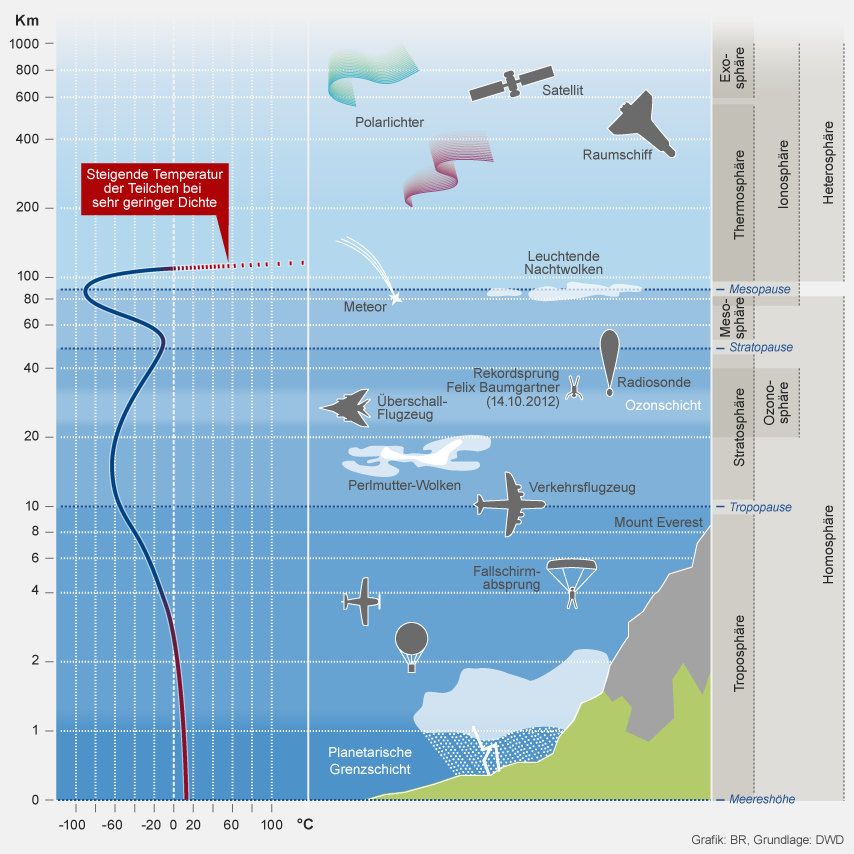
\includegraphics[width=8cm]{meteorologie-wetter-atmosphaere-102}

\subsection{Auftrieb}
\subsubsection{Flügelgeometrie}

\begin{itemize}
    \item Zuspitzung: $\lambda = \frac{c_t}{c_0}$
    \item Flügelfläche: $F = \int_{-b/2}^{b/2} c(y) dy$ 
    \item Streckung: $\Lambda = b^2 /F$
    \item Mittl. geome. Flügeltiefe: $\overline{c} = \frac{1}{b} \int_{-b/2}^{b/2} c(y) dy = F/b$ 
    \item Mittl. aero. Flügeltiefe: $l_\mu = \frac{1}{F} \int_{-b/2}^{b/2} c^2(y) dy $
    \item Geometrischer Neutralpunkt = Ort wo die Änderung des Anstellwinkels keine Auswirkung auf Kraft und Moment hat
    \item $x_{N25} = \frac{1}{F} \int_{-b/2}^{b/2} c^2(y) x_{25}(y) dy \approx x_{c_0/4}$, $y_{N25} = 0$
\end{itemize}

Achtung: $b_{ges} = 2\cdot b_{flugel}$!

\begin{center}
    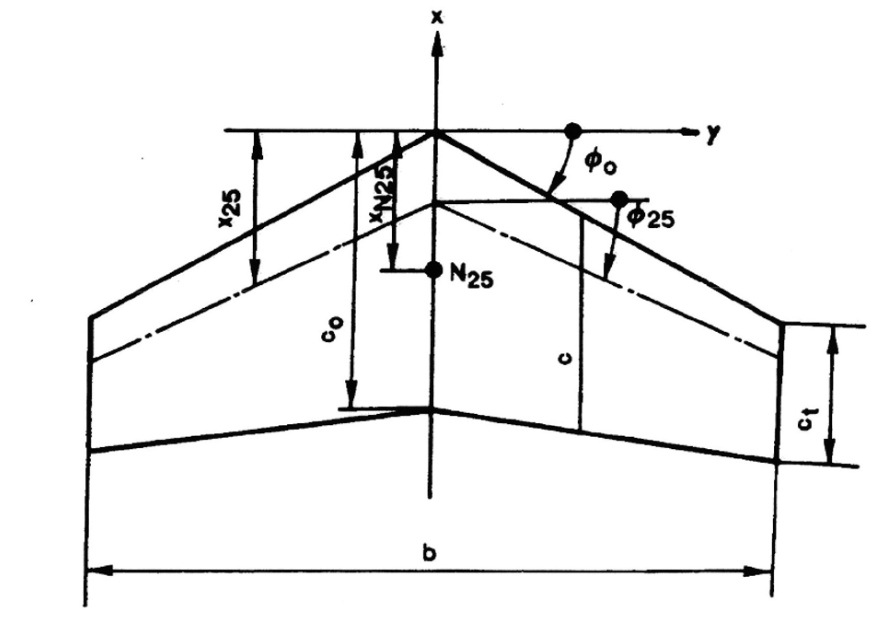
\includegraphics[width = 6cm]{Fluegelgeometrie-1.png}
\end{center}
\begin{tabular}{ l | l l l l}
    & Recht & Trapez & Dreieck & Ellipse \\ 
    \hline
    F & $bc$ & $\frac{c_0+c_t}{2}b$ & $\frac{c_0}{2}b$ & $\frac{\pi}{4}b c_0$ \\ 
    \hline 
    $\Lambda$ & $b/c$ & $2b/(c_0+c_t)$ & $2b/c_0$ & $4b/(\pi c_0)$ \\
    \hline
    $\lambda$ & $1$ & $c_t/c_0$ & 0 & - \\
    \hline
    $\overline{c}$ & c & $(c_0+c_t)/2$ & $c_0/2$ & $\pi/4$ \\
    \hline
    $l_\mu$ & c & $\frac{2}{3}\frac{c_0^2+c_0c_t+c_t^2}{c_0+c_t}$ & $2c_0/3$ & $\frac{8}{3\pi}c_0$ \\
    \hline
    $x_{25}$ & $c/4$ & $\frac{c_0}{4}+\frac{c_0 b}{6(c_0+c_t)}(1+\frac{2c_t}{c_0})tg(\phi_{25})$ & $\frac{c_0}{4}\frac{b}{6}tg(\phi_{25})$ & $\frac{c_0}{4}\frac{b}{6}tg(\phi_{25})$ \\
    \hline
\end{tabular}

\subsubsection{Flügelprofile}

\begin{tabular}{l | l l }
    & Flügel (3D) & Profil (2D) \\ 
    \hline
    Auftrieb & $c_A = \frac{A}{\frac{1}{2}\rho V^2 F}$& $c_a = \frac{A'}{\frac{1}{2}\rho V^2 c}$  \\
    \hline
    Widerstand & $c_W = \frac{W}{\frac{1}{2}\rho V^2 F}$ & $c_w = \frac{W'}{\frac{1}{2}\rho V^2 c}$ \\
    \hline
    Nickmoment & $c_M = \frac{M}{\frac{1}{2}\rho V^2 F l_\mu}$ & $c_m = \frac{M'}{\frac{1}{2}\rho V^2 c^2}$\\
    \hline
\end{tabular}
\newline \newline
Hierbei sind Grössen mit Apostroph pro Spannbreite berechnet (Kraft/Moment pro $b$)

\begin{itemize}
    \item \textbf{Auftriebspolaren:} Nullauftriebswinkel $\alpha_0$ (Winkel wo aerodyn. Auftrieb verschwindet)
    \item $\alpha_0 = 0$ für symmetrische Profile
    \item $\alpha_0 < 0$ für gewölbte Profile
    \item \textbf{Linearbereich}
    \item $c_a = \frac{dc_a}{d\alpha}(\alpha-\alpha_0)$ mit Auftriebsgradient 
    \item $\frac{dc_a}{d\alpha}$: Konstant im Linearbereich
    \item \textbf{Maximaler Auftriebsbeiwert:} $c_{a,max}$ bestimmt die Abrissgeschwindigkeit
    \item \textbf{Minimaler Auftriebsbeiwert:} $c_{a,min}$ analog wie $c_{a,max}$ im Rückenflug
\end{itemize}


\subsection{Widerstand}

\section{Einführung in die Fahrzeugaerodynamik}


\subsection{Grundlagen}

\subsection{Personenwagen}

\subsection{Nutzfahrzeuge}

\subsection{Rennfahrzeuge}


\end{multicols*}
\end{document}

